% !TEX root = short.tex
% !TEX program = lualatex

% The 8-page version of the internal report (Hani's request of 2026-11-11; the request
% and the plan: archive/tampura_bridge_plan_2026-10-25/tracks/report/short/REQUEST.md).
% The full report stays in main.tex, untouched. This file shares resources/preamble.tex
% and overrides only the layout, here, so that the preamble itself is not edited.

% !TEX root = ../main.tex

% DO NOT TOUCH! unless absolutely necessary (consider updating the template then)

\documentclass[11pt, oneside]{book} % TODO add 'final' option once document is complete
\usepackage[a4paper,
            width=150mm,
            top=35mm,
            bottom=35mm,
            bindingoffset=10mm,
            marginparwidth=30mm,
            headheight=5mm,
            headsep=10mm,
            footskip=15mm,
            hcentering]{geometry}
\usepackage[backend=biber, sorting=nyt, citestyle=numeric-comp, bibstyle=ieee, maxbibnames=999]{biblatex}
\usepackage[ngerman, american]{babel}
\usepackage{setspace}
\usepackage{fancyhdr}
\usepackage[pdfusetitle, hidelinks]{hyperref}
\usepackage{mathtools}
\usepackage[warnings-off={mathtools-colon,mathtools-overbracket}]{unicode-math}
\usepackage{amsthm}
\usepackage{upgreek}
\usepackage{nicefrac}
\usepackage{algorithm}
\usepackage[beginComment=, beginLComment=, endLComment=]{algpseudocodex}
\usepackage{listings}
\usepackage{mleftright}
\usepackage{graphicx}
\usepackage{csquotes}
\usepackage{parskip}
\usepackage{titlesec}
\usepackage{xcolor}
\usepackage{lipsum}
\usepackage{pgfplots}
\usepackage{tikzpagenodes}
\usepackage{bookmark}
\usepackage{xurl}
\usepackage{etoolbox}
\usepackage{comment}
\usepackage{booktabs}
\usepackage{tabularx}
\usepackage{longtable}
\usepackage{emptypage}
\usepackage{letltxmacro}
\usepackage[all]{nowidow}
\usepackage[final]{microtype}
\usepackage[nottoc]{tocbibind}
\usepackage[shortcuts]{extdash}
\usepackage[detect-all]{siunitx}
\usepackage[skip=5pt]{subcaption}
\usepackage[obeyFinal]{todonotes}
\usepackage[shortlabels]{enumitem}
\usepackage[nodayofweek]{datetime}
\usepackage{epigraph}
\usepackage{totcount}
\usepackage[figure,table,lstlisting,algorithm]{totalcount}
\usepackage[capitalize, nameinlink, noabbrev]{cleveref}
\usepackage[format=hang, font={color=darkgray, singlespacing}, skip=5pt]{caption}
\usepackage[lang-warn=false]{datatool-base}
\usepackage[style=alttree, acronym, symbols, nomain, nonumberlist, shortcuts=ac]{glossaries-extra}

% custom macros
% !TEX root = ../main.tex

% math typesetting utilities
\newcommand*{\given}{\;\middle|\;}
\newcommand*{\hateq}{\mathrel{\widehat{=}}}
\newcommand*{\tuple}[1]{\left\langle #1 \right\rangle}
\newcommand*{\set}[1]{\left\{ #1 \right\}}
\newcommand*{\multiset}[1]{\left\{\!\left\{ #1 \right\}\!\right\}}
\newcommand*{\evalat}[2][]{\left. #2 \right\rvert_{#1}}
\newcommand*{\bmat}[1]{\begin{bmatrix} #1 \end{bmatrix}}
\newcommand*{\sbmat}[1]{\begin{bsmallmatrix} #1 \end{bsmallmatrix}}
\newcommand*{\dbmat}[1]{\everymath{\displaystyle} \begin{bmatrix} #1 \end{bmatrix}}
\newcommand*{\abs}[1]{\left\lvert #1 \right\rvert}
\newcommand*{\norm}[1]{\left\lVert #1 \right\rVert}
\newcommand*{\bvec}[1]{{\symbfit{#1}}}

% math operators
\DeclareMathOperator*{\argmax}{arg\,max}
\DeclareMathOperator*{\argmin}{arg\,min}
\DeclareMathOperator*{\Exp}{\symbb{E}}
\DeclareMathOperator*{\Prob}{\symbb{P}}
\newcommand*{\expectation}[2][]{\Exp_{#1} \left[ #2 \right]}
\newcommand*{\probability}[1]{\Prob \left[ #1 \right]}

% environments
\newtheorem{theorem}{Theorem}
\newtheorem{problem}{Problem} \crefname{problem}{Problem}{Problems}
\newtheorem{hypothesis}{Hypothesis} \crefname{hypothesis}{Hypothesis}{Hypotheses}

% report only: internal source tags. A tag names the PAPER_AUDIT.txt entry (or
% another internal document) a number or finding comes from, and links to its
% row in the appendix "Internal sources" (\isrcrow makes the link target there).
\newcommand*{\BF}[1]{\hyperlink{src:BF#1}{BF\#{}#1}}
\newcommand*{\PW}[1]{\hyperlink{src:P#1}{\#P#1}}
\newcommand*{\TK}[1]{\hyperlink{src:TK#1}{path~#1}}
\newcommand*{\ID}[2]{\hyperlink{src:#1}{#2}}
\newcommand*{\isrcrow}[5]{\hypertarget{src:#1}{#2} & #3 & #4 & #5 \\}

% graphics directory
\graphicspath{{figures/}{../thesis/graphics/}}

% bibtex references
\addbibresource{../thesis/resources/references.bib}
\addbibresource{resources/report_extra.bib}

% acronym and symbol counters
\newtotcounter{acronyms}
\glsdefpostlink{acronym}{\glsxtrifwasfirstuse{\stepcounter{acronyms}}{}}
\newtotcounter{symbols}
\def\oldglsxtrnewsymbol{} \let\oldglsxtrnewsymbol=\glsxtrnewsymbol
\def\glsxtrnewsymbol{\stepcounter{symbols}\oldglsxtrnewsymbol}

% acronyms and symbols glossary
\makenoidxglossaries
\glspatchtabularx
\setabbreviationstyle[acronym]{long-short}
\loadglsentries{resources/acronyms.tex}
\setglossarypreamble[acronym]{
  \glssetwidest{TAMPURA\;\;\:}
  \setlength{\parskip}{0pt}
}
\glsxtrprovidestoragekey{group}{}{\glsgroup}
\newcommand*{\newglsgroup}[2]{\glsxtrnewsymbol[description={}, group=#1]{group-#1}{\textbf{#2}}}
\loadglsentries{resources/symbols.tex}
\setglossarypreamble[symbols]{
  \glssetwidest{\ensuremath{\argmax_a f(a)}\;\;\:}
  \setlength{\parskip}{0pt}
  \let\glsnamefont\textnormal
}

% fonts: the thesis's font files are used from ../thesis/fonts/ without copying them;
% .latexmkrc puts that folder on kpathsea's font search path (TTFONTS), because LuaTeX
% fails (cannot find file '') on a font loaded through a Path= that leaves this folder.
\setmainfont{STIXTwoText}[
  Extension=.ttf,
  UprightFont={*-Regular},
  BoldFont={*-Bold},
  ItalicFont={*-Italic},
  BoldItalicFont={*-BoldItalic}
]
\setmathfont{STIXTwoMath}[
  Extension=.ttf,
]
\setsansfont{NotoSans}[
  Extension=.ttf,
  UprightFont={*-Regular},
  BoldFont={*-Bold},
  ItalicFont={*-Italic},
  BoldItalicFont={*-BoldItalic},
  Scale=MatchLowercase
]
\setmonofont{NotoSansMono}[
  Extension=.ttf,
  UprightFont={*-Regular},
  BoldFont={*-Bold},
  ItalicFont={*-Regular},
  BoldItalicFont={*-Bold},
  ItalicFeatures=FakeSlant,
  Scale=MatchLowercase
]

% line spacing
\onehalfspacing
\setlist{nosep}

% page layout
\pagestyle{fancy}
\fancyhf{}
\makeatletter
\if@twoside
  \fancyhead[LE]{\nouppercase{%
    \if@mainmatter \thechapter\enskip \fi
    \leftmark
  }}
  \fancyhead[RO]{\nouppercase{%
    \if@mainmatter \thesection\enskip \fi
    \rightmark
  }}
  \fancyfoot[LE,RO]{\thepage}
\else
  \fancyhead[R]{\nouppercase{%
    \if@mainmatter \thechapter\enskip \fi
    \leftmark
  }}
  \fancyfoot[R]{\thepage}
\fi
\fancypagestyle{plain}{
  \fancyhf{}
  \fancyfoot[R]{\thepage}
  \renewcommand{\headrulewidth}{0pt}
}
\fancypagestyle{title}{
  \fancyhf{}
  % report: no footer on the title page (the thesis prints place and date here);
  % the date of the state is the "State of ..." line of the title page itself
  \renewcommand{\headrulewidth}{0pt}
}
\makeatother
\renewcommand{\chaptermark}[1]{\markboth{#1}{}}
\renewcommand{\sectionmark}[1]{\markright{#1}}

% chapter layout
\titlespacing*{\chapter}{0pt}{0pt}{10mm}
\titleformat{\chapter}[hang]{\huge\bf}{\thechapter}{1em}{\huge}

% custom abstract environment
\newenvironment{abstract}{
  \chapter*{Abstract}
}{
  \glsresetall
}

% report only: unnumbered Summary and Preface chapters, listed in the contents
\newenvironment{summary}{
  \chapter*{Summary}
  \addcontentsline{toc}{chapter}{Summary}
}{
  \glsresetall
}
\newenvironment{preface}{
  \chapter*{Preface}
  \addcontentsline{toc}{chapter}{Preface}
}{
  \glsresetall
}
% float placement
\makeatletter
\setlength{\@fptop}{0pt}
\setlength{\@fpsep}{17pt}
\makeatother
\raggedbottom

% todonotes layout
\reversemarginpar
\setuptodonotes{
  size=\footnotesize,
  backgroundcolor=white,
  linecolor=gray,
  bordercolor=gray,
  tickmarkheight=5pt
}
\let\TODO\todo

% pgfplot version specification
\pgfplotsset{compat=1.18}

% math parentheses spacing adjustments
\mleftright

% inline math line break prevention
\binoppenalty=10000
\relpenalty=10000

% remap (, ), [, and ] to \left(, \right), \left[, and \right]
\begingroup
  \catcode`(\active \xdef({\left\string(}
  \catcode`)\active \xdef){\right\string)}
  \catcode`[\active \xdef[{\left\string[}
  \catcode`]\active \xdef]{\right\string]}
\endgroup
\mathcode`(="8000 \mathcode`)="8000
\mathcode`[="8000 \mathcode`]="8000

% algorithm settings
\algrenewcommand\alglinenumber[1]{\color{gray}\footnotesize #1\enspace}

% listings settings
\lstset{
  basicstyle={\ttfamily\singlespacing},
  frame=lines,
  numbers=left,
  numberstyle={\color{gray}\ttfamily\footnotesize},
  xleftmargin=7mm,
  framexleftmargin=7mm,
  belowcaptionskip=\dimexpr-0.8244023083\baselineskip+8.5pt\relax,
  showstringspaces=false,
  commentstyle={\color{gray}\itshape}
}
\renewcommand{\lstlistlistingname}{List of Listings}

% Listing style for PDDL
% The generic Lisp lexer only caught comments and a couple of operators
% (and/not).  This dedicated PDDL language additionally highlights the
% :keywords, the logical operators, the type predicates, and the
% ?-variables, so the structure of an action (parameters / precondition /
% effect) and its variables stand out.
\definecolor{pddlkw}{RGB}{0,0,190}       % structural / :keywords
\definecolor{pddlop}{RGB}{150,30,150}    % logical operators
\definecolor{pddltype}{RGB}{0,120,120}   % type predicates
\definecolor{pddlvar}{RGB}{200,85,0}     % ?-variables
\lstdefinelanguage{PDDLlang}{
    alsoletter={?:-_},
    sensitive=true,
    morecomment=[l]{;},
    morestring=[b]",
    morekeywords=[1]{define,domain,problem,stream,:requirements,:strips,
      :equality,:typing,:derived-predicates,:conditional-effects,
      :action-costs,:predicates,:functions,:action,:parameters,
      :precondition,:effect,:derived,:stream,:inputs,:outputs,:certified,
      :domain,:init,:goal,:objects,:fluents},
    morekeywords=[2]{and,or,not,when,forall,exists,imply,increase,decrease,either},
    morekeywords=[3]{Boxel,Obj,Config,Trajectory,Grasp},
    morekeywords=[4]{?x,?b,?obj,?region,?o,?o1,?o2,?on_obj,?q,?q1,?q2,?t,?g},
}
\lstdefinestyle{PDDL}{
    language=PDDLlang,
    basicstyle=\ttfamily\footnotesize, % Font style and size
    keywordstyle=[1]\color{pddlkw}\bfseries,  % structural / :keywords
    keywordstyle=[2]\color{pddlop},            % logical operators
    keywordstyle=[3]\color{pddltype},          % type predicates
    keywordstyle=[4]\color{pddlvar},           % ?-variables
    commentstyle=\color{green!60!black}\itshape, % Green and italic comments
    stringstyle=\color{purple}, % Purple strings
    showstringspaces=false, % Don't show spaces in strings
    breaklines=true, % Allow line breaks within code
    breakatwhitespace=true, % Break lines at whitespace
    tabsize=2, % Tab size
    captionpos=b, % Caption below the listing
    escapeinside={\%*}{*)} % Allows LaTeX commands inside listings
}

% conditional lists
\newcommand{\listacronyms}{
  \ifnum\totvalue{acronyms}>0
    \printnoidxglossary[type=acronym, title={List of Acronyms}]
  \fi
}
\newcommand{\listsymbols}{
  \ifnum\totvalue{symbols}>0
    \printunsrtglossary[type=symbols, title={List of Symbols}]
  \fi
}
\newcommand{\listfigures}{
  \iftotalfigures
    \listoffigures
  \fi
}
\newcommand{\listtables}{
  \iftotaltables
    \listoftables
  \fi
}
\newcommand{\listalgorithms}{
  \iftotalalgorithms
    \listofalgorithms\addcontentsline{toc}{chapter}{List of Algorithms}
  \fi
}
\newcommand{\listlistings}{
  \iftotallstlistings
    \lstlistoflistings\addcontentsline{toc}{chapter}{List of Listings}
  \fi
}
\newcommand{\listreferences}{
  \emergencystretch=1em
  \printbibliography[title={List of References}, heading=bibintoc]
}
\newcommand{\listtodos}{
  \ifnum\value{@todonotes@numberoftodonotes}>0
    \listoftodos[List of TODOs]
  \fi
}

% SI units settings
\robustify\bfseries
\sisetup{list-final-separator=\text{, and }}

% citation settings
\newcommand{\creflastconjunction}{, and }


% ---- layout of the short version (overrides of the shared preamble) ----
\geometry{reset, a4paper, hmargin=17mm, top=17.5mm, bottom=13mm,
          headheight=5mm, headsep=4mm, footskip=7mm}
\makeatletter
\renewcommand\normalsize{\@setfontsize\normalsize{9.6pt}{11.6pt}%
  \abovedisplayskip 5pt plus 2pt minus 3pt \belowdisplayskip\abovedisplayskip
  \abovedisplayshortskip 0pt plus 2pt \belowdisplayshortskip 3pt plus 2pt minus 2pt
  \let\@listi\@listI}
\renewcommand\small{\@setfontsize\small{8.6pt}{10.3pt}}
\renewcommand\footnotesize{\@setfontsize\footnotesize{7.8pt}{9.3pt}}
\renewcommand\scriptsize{\@setfontsize\scriptsize{6.8pt}{8.1pt}}
% source tags print as plain text: the short version has no appendix to link to
\src@plaintrue
\makeatother
\singlespacing
\normalsize
\setlength{\parskip}{2.5pt plus 1pt}
\setlength{\parindent}{0pt}

\setcounter{secnumdepth}{1}
\renewcommand\thesection{\arabic{section}}
\renewcommand\thefigure{\arabic{figure}}
\renewcommand\thetable{\arabic{table}}
\titleformat{\section}{\normalfont\large\bfseries}{\thesection}{0.6em}{}
\titlespacing*{\section}{0pt}{7pt plus 2pt}{2pt}
\titleformat{\paragraph}[runin]{\normalfont\bfseries}{}{0pt}{}
\titlespacing*{\paragraph}{0pt}{3pt}{0.5em}

\pagestyle{fancy}
\fancyhf{}
\fancyhead[L]{\footnotesize\color{darkgray}Semantic Boxels since the thesis: Checkpoint 1 in eight pages}
\fancyhead[R]{\footnotesize\color{darkgray}\thepage}
\renewcommand{\headrulewidth}{0.3pt}

\captionsetup{font={footnotesize, color=darkgray, singlespacing}, skip=3pt}
\captionsetup[sub]{font={scriptsize, color=darkgray}, skip=2pt}
\setlength{\textfloatsep}{6pt plus 2pt}
\setlength{\floatsep}{5pt plus 2pt}
\setlength{\intextsep}{5pt plus 2pt}
\setlist{nosep, leftmargin=1.2em}
\renewcommand{\arraystretch}{1.1}

% colours: ours and TAMPURA as in the full report's figure; verdict marks
\colorlet{cours}{blue!55!black}
\colorlet{ctamp}{orange!85!black}
\colorlet{vok}{green!45!black}
\colorlet{vnarrow}{orange!75!black}
\colorlet{vrerun}{red!70!black}
\colorlet{vnot}{black!55}
\newcommand*{\vOK}{\textcolor{vok}{\textbf{valid}}}
\newcommand*{\vNA}{\textcolor{vnarrow}{\textbf{narrower}}}
\newcommand*{\vRE}{\textcolor{vrerun}{\textbf{re-run}}}
\newcommand*{\vNO}{\textcolor{vnot}{\textbf{not run}}}

\pgfplotsset{
  sb/.style={
    tick label style={font=\scriptsize}, label style={font=\scriptsize},
    legend style={font=\scriptsize, draw=none, fill=none, legend cell align=left,
                  /tikz/every even column/.append style={column sep=4pt}},
    grid style={black!12}, axis line style={black!55}, tick style={black!55},
    xlabel shift=-3pt, ylabel shift=-3pt,
  },
}

% small marks: a verdict square for the timeline, status dots for the track matrix
\newcommand*{\sq}[1]{\textcolor{#1}{\rule{1.15ex}{1.15ex}}\hspace{0.35em}}
\newcommand*{\dY}{\tikz[baseline=-0.6ex]\fill[cours] (0,0) circle (2.4pt);}
\newcommand*{\dH}{\tikz[baseline=-0.6ex]{\draw[cours, line width=0.5pt] (0,0) circle (2.4pt);
  \fill[cours] (0,-2.4pt) arc[start angle=-90, end angle=90, radius=2.4pt] -- cycle;}}
\newcommand*{\dN}{\tikz[baseline=-0.6ex]\draw[black!45, line width=0.5pt] (0,0) circle (2.4pt);}

% one tile of the failure gallery: frame colour, scene number, label
\newcommand*{\tile}[3]{\begin{minipage}[t]{0.157\linewidth}\centering
  {\setlength{\fboxsep}{0pt}\setlength{\fboxrule}{1.3pt}%
   \fcolorbox{#1}{white}{\includegraphics[width=\dimexpr\linewidth-2.6pt\relax]{short/fail_tile_s#2.png}}}\par
  \vspace{1pt}{\scriptsize\color{darkgray}\textbf{#2}: #3\par}\end{minipage}}

% the archive, as seen from report/
\newcommand*{\arch}{../archive/tampura_bridge_plan_2026-10-25}

\begin{document}

{\footnotesize\bfseries\color{darkgray}Internal Report\quad\textbullet\quad Checkpoint 1\quad\textbullet\quad
Short version (8 pages) of Version 2 (84 pages)}\par
\vspace{1pt}
{\LARGE\bfseries Semantic Boxels Since the Thesis: The State in Eight Pages}\par
\vspace{2pt}
{\small State of 8 November 2026\quad\textbullet\quad written 12 November 2026\quad\textbullet\quad Hani Alassiri Alhabboub}\par
\vspace{3pt}\hrule\vspace{4pt}

\section{The answers in short}
\label{sec:answers}

\begingroup\small
\begin{tabularx}{\linewidth}{@{}P{0.20\linewidth}Y@{}}
\textbf{What was achieved?} &
An honest system (no weld, perception from rendered images); a die that stays in the hand (120 of 120 episodes); a
first comparison with TAMPURA on fresh scenes, ahead and not significant; a known cause of our failures; and from
the tracks the mirror experiment, LW1 in a 3-D Wumpus world, two more tasks and a bug board (\Cref{sec:achieved}). \\
\textbf{What was changed?} &
The numbers measured the tag \texttt{stable-2026-11-06}. Since then only a launcher fix and the boxel drawing were
merged. Everything else sits on nine unmerged branches, and the main checkout carries three uncommitted fix hunks
(\Cref{sec:changed}). \\
\textbf{What was tested?} &
48 runs and checks are on record: the cluster evaluations up to 4 November and the tracks' laptop runs of 6 to 8
November. Nothing has run on the cluster since the tracks began, and no evaluation has run since the rule of 8
November that asks for drop and collision counts (\Cref{sec:tested}). \\
\textbf{What is not valid?} &
Two runs have to be run again: the first arm of path 7, which ran before its deviations were approved, and the
hand-camera batch of the mirror, cut at 2 of 10 seeds. Twenty-one results stand only for a narrower claim. Among
them are the mirror (ours 10 of 10 against TAMPURA 6 of 10), confounded by our fixed camera and to be repeated,
and both comparisons with TAMPURA: each arm by its own end test, drops not recorded. No old record can be
re-scored for drops (\Cref{sec:tested}). \\
\textbf{Laptop or cluster?} &
Laptop only: everything Hani must watch, the A/B of the drop cure, the mirror, the Wumpus runs and the first run of
the shared success test. Cluster: every comparison whose number or time goes into the paper, all arms on one node
type, after Hani's yes to that question alone (\Cref{sec:placement}). \\
\textbf{What stopped right before it was done?} &
The A/B of the drop cure (50 minutes), eight seeds of TAMPURA with its own hand camera, the waiting merges, and the
first real run of the shared success test. The cluster evaluation and path 8 are further from done than the
tracks' state suggests (\Cref{sec:stopped}). \\
\textbf{What is missing?} &
Drop and collision counts in our pipeline, one success test for both arms, a frozen code version for the paper,
Hani's written approvals, the cluster comparison on 200 fresh scenes, and a decision on the die under the cup
(\Cref{sec:missing}). \\
\textbf{What is quick?} &
Four things take Hani less than an hour together and unblock most of the rest; about ten more take an agent less
than a day each (\Cref{sec:quick}). \\
\end{tabularx}
\endgroup

\begin{figure}[H]
\centering
\begin{subfigure}[t]{0.19\linewidth}\centering
  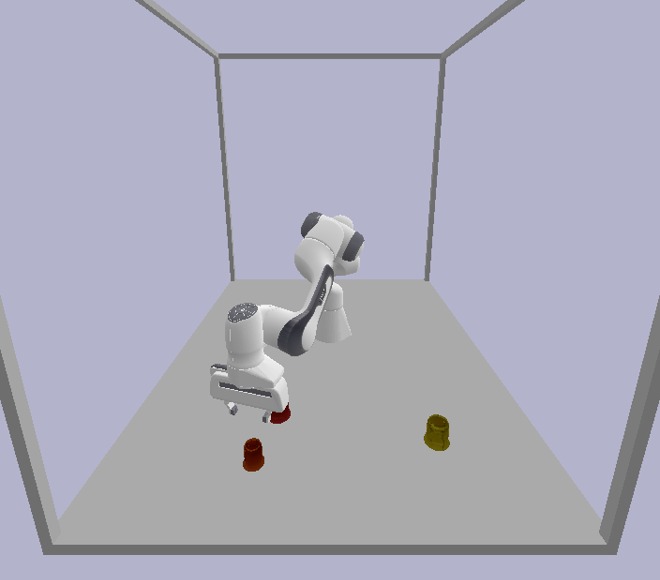
\includegraphics[width=\linewidth]{short/fd_ours_s10_frame025.png}
  \caption{Ours in TAMPURA's \fdice\ world, at a cup (GUI run, 30 Oct, seed 10).}
\end{subfigure}\hfill
\begin{subfigure}[t]{0.19\linewidth}\centering
  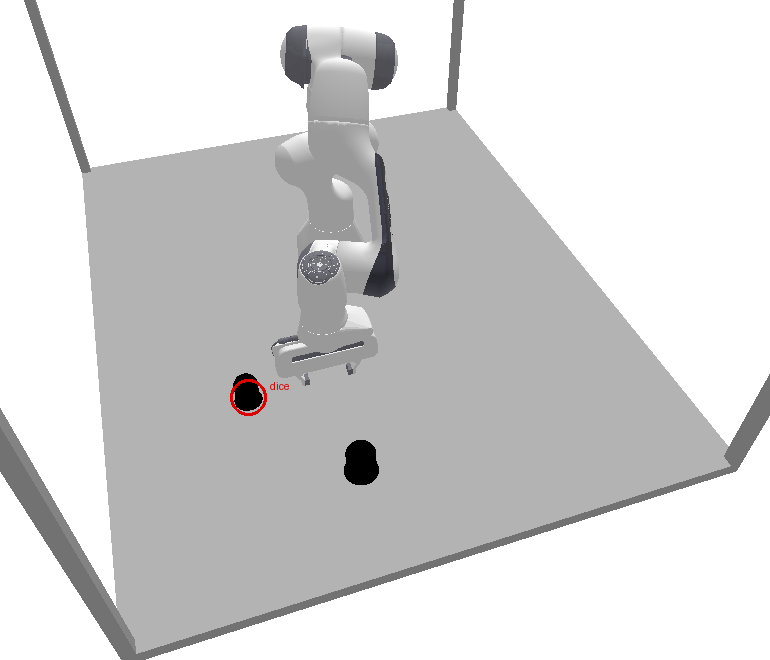
\includegraphics[width=\linewidth]{short/fd_fail_s118_overview.png}
  \caption{A failure of ours on a generated scene (118): the die (ring) sits under a cup that casts no searched shadow.}
\end{subfigure}\hfill
\begin{subfigure}[t]{0.19\linewidth}\centering
  \includegraphics[width=\linewidth]{\arch/tracks/reverse/batch1/failed_T/s3_final_view.png}
  \caption{The mirror: TAMPURA's planner on our scene, seed 3, at its end, a box still in the hand.}
\end{subfigure}\hfill
\begin{subfigure}[t]{0.19\linewidth}\centering
  \includegraphics[width=\linewidth]{\arch/tracks/reverse/batch_hand_c/first_views/s0_first_view_hand.png}
  \caption{TAMPURA's own hand camera, first image on seed 0: one of three objects, not the target.}
\end{subfigure}\hfill
\begin{subfigure}[t]{0.19\linewidth}\centering
  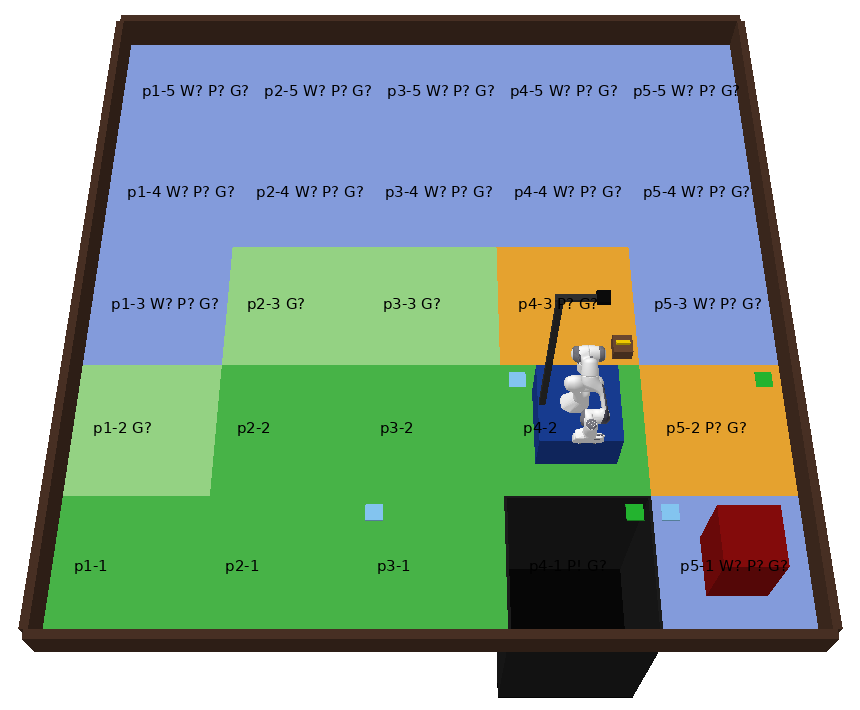
\includegraphics[width=\linewidth]{short/wumpus_lw1_frame006.png}
  \caption{LW1 drives our robot in the 3-D Wumpus world (5x5, after 13 actions; tiles coloured by what is known).}
\end{subfigure}
\caption{Five of the settings that were run. All images are from archived runs; none was made for this report.}
\label{fig:shots}
\end{figure}

\section{What was achieved}
\label{sec:achieved}

Since the thesis was handed in on 10 June 2026:
\begin{itemize}
\item \textbf{The system no longer cheats in grasping and perception.} The weld that held every object is gone and
the gripper holds by friction, with a squeeze of 0.5\,mm since 30 October (\BF{44}); detection reads rendered images;
failures of the physics are detected and reported as failures; 32 field findings were fixed or recorded (\PW{1}, \PW{2}).
\item \textbf{The comparison with TAMPURA was rebuilt on an honesty contract.} The first bridge reported 20 of 20
because its code chose the cup, welded the grasp and wrote success into TAMPURA's belief; it was thrown away on 20
August. Since 25 October our perception, belief, planner and physical execution run inside TAMPURA's \fdice\ world
under automated gates and a run ledger. Four adversarial reviewers found no cheat; their 37 findings led to nine gate
fixes (\BF{14} to \BF{25}).
\item \textbf{The die no longer slips out of the hand.} Six fixes ran as switches. The chosen four gave 120 of 120
episodes over two jobs and no die lost in 120 carries, against 209 of 300 without them and 40 of 60 for TAMPURA, on
the three scenes that TAMPURA ships (\Cref{fig:fd}a). They are on by default since 2 November (\BF{59}, \BF{62}).
\item \textbf{A comparison on fresh scenes exists.} On 40 scenes from TAMPURA's own generator ours solved 57 of 80 and
TAMPURA 46 of 76, with pairs 18 to 9 and exact McNemar $p = 0.12$: ahead, not significant (\Cref{fig:fd}b,
\Cref{fig:pairs}a). Our runs of TAMPURA land near its paper: a return of 0.530 against the published
0.63 $\pm$ 0.07 (\BF{63}).
\item \textbf{We know why we fail there.} Ours fails on 23 episodes in each run, in the same 12 scenes, with no die
lost. In 16 of the 17 that ended with all shadows searched, the shadow behind the cup was clipped away (\BF{64}; the
fix is checked on a branch). Beneath that lies a limit of the representation: the die under a cup lies in none of our
hiding regions, and every success of ours on \fdice\ came from lifting a cup, never from a sensing action
(\BF{65}, \Cref{fig:shots}b).
\item \textbf{Episodes got shorter.} Of four time cuts only the planner's search settings helped: the median wall
time fell from 34.6 to 23.2\,s (\BF{53}, \BF{57}).
\item \textbf{Three days of parallel tracks (6 to 8 November) added:} the mirror experiment, TAMPURA's planner on our
scenes (\Cref{fig:pairs}b); the classical planner LW1 driving our robot through a 3-D Wumpus world, 18 of 18 episodes
with 0 of 369 percepts wrong, and the luck floor of that test (\Cref{fig:other}a); our planning layer alone on two
more TAMPURA tasks (\Cref{fig:other}b); a board of 23 bugs with four fixes ready to merge; the drop bug TB-23 with two
causes and a candidate cure (\Cref{fig:pairs}c); a correction of the thesis (25 of the 29 ``timeouts'' on stack ended
after 8 to 21\,s, rejected by the end-of-run physics check, \BF{68}); and reports on the WSL wedge (\BF{69}) and on
21.3\,GB of dead data.
\end{itemize}

\begin{figure}[H]
\centering
\begin{subfigure}[t]{0.50\linewidth}\centering
\begin{tikzpicture}
\begin{axis}[sb, xbar, bar width=5.2pt, width=0.72\linewidth, height=4.8cm,
  xmin=0, xmax=128, xtick={0,25,50,75,100},
  xlabel={successes of counted episodes (\%)},
  symbolic y coords={tampura,base,iters,pose,check,poseyaw,itersforce,accel,chosen},
  ytick={tampura,base,iters,pose,check,poseyaw,itersforce,accel,chosen},
  yticklabels={{TAMPURA},{our base, four jobs},{more solver iterations},{pose uncertainty kept},{hold check},{pose kept, yaw near home},{iterations, force hold},{pose, yaw, limited accel.},{\textbf{the chosen set of four}}},
  enlarge y limits=0.07,
  nodes near coords, point meta=explicit symbolic,
  nodes near coords style={font=\scriptsize, anchor=west},
  xmajorgrids,
]
\addplot[fill=cours, draw=none, bar shift=0pt] coordinates {(70.0,base) [168/240] (43.3,iters) [26/60] (65.0,pose) [39/60] (70.0,check) [42/60] (81.7,poseyaw) [49/60] (90.0,itersforce) [54/60] (90.0,accel) [54/60] (100,chosen) [60/60]};
\addplot[fill=ctamp, draw=none, bar shift=0pt] coordinates {(66.7,tampura) [40/60]};
\end{axis}
\end{tikzpicture}
\caption{The die-slip campaign on the three shipped scenes (\BF{59}): each fix alone and in sets. A second job repeated the chosen set: 60 of 60 again.}
\end{subfigure}\hfill
\begin{subfigure}[t]{0.47\linewidth}\centering
\begin{tikzpicture}
\begin{axis}[sb, ybar, bar width=7pt, width=\linewidth, height=4.8cm,
  ymin=0, ymax=135, ytick={0,25,50,75,100},
  ylabel={successes (\%)}, xlabel={cups in the scene},
  symbolic x coords={1,2,3,4,5}, xtick=data, enlarge x limits=0.14,
  legend style={at={(0.5,1.02)}, anchor=south, legend columns=2},
  nodes near coords, point meta=explicit symbolic,
  nodes near coords style={font=\scriptsize, rotate=90, anchor=west},
  ymajorgrids,
]
\addplot[fill=cours, draw=none] coordinates {(1,100) [14/14] (2,55.6) [10/18] (3,62.5) [10/16] (4,75) [12/16] (5,68.8) [11/16]};
\addplot[fill=ctamp, draw=none] coordinates {(1,100) [12/12] (2,62.5) [10/16] (3,62.5) [10/16] (4,37.5) [6/16] (5,50) [8/16]};
\legend{ours, TAMPURA}
\end{axis}
\end{tikzpicture}
\caption{Run 2 on 40 generated scenes by number of cups (\BF{63}): ours 57 of 80, TAMPURA 46 of 76.}
\end{subfigure}
\caption{Ours against TAMPURA on \fdice, on the cluster. Success is each arm's own end test.}
\label{fig:fd}
\end{figure}

\begin{figure}[H]
\centering
\begin{subfigure}[t]{0.37\linewidth}\centering
\begin{tikzpicture}
\begin{axis}[sb, xbar, bar width=4.6pt, width=0.66\linewidth, height=4.2cm,
  xmin=0, xmax=82, xtick={0,20,40,60},
  xlabel={dice lost per carry home (\%)},
  symbolic y coords={base,iters,pose,check,poseyaw,itersforce,accel,chosen},
  ytick={base,iters,pose,check,poseyaw,itersforce,accel,chosen},
  yticklabels={{our base, four jobs},{more solver iterations},{pose uncertainty kept},{hold check},{pose kept, yaw near home},{iterations, force hold},{pose, yaw, limited accel.},{\textbf{the chosen set of four}}},
  enlarge y limits=0.08,
  nodes near coords, point meta=explicit symbolic,
  nodes near coords style={font=\scriptsize, anchor=west},
  xmajorgrids,
]
\addplot[fill=vrerun, draw=none] coordinates {(19.2,base) [40/208] (54.4,iters) [31/57] (33.9,pose) [20/59] (17.6,check) [9/51] (2.0,poseyaw) [1/50] (0,itersforce) [0/54] (0,accel) [0/54] (0,chosen) [0/60]};
\end{axis}
\end{tikzpicture}
\caption{The die-slip campaign again: dice lost in the hand per carry, as the pipeline noticed them (\BF{59}).}
\end{subfigure}\hfill
\begin{subfigure}[t]{0.27\linewidth}\centering
\begin{tikzpicture}
\begin{axis}[sb, width=\linewidth, height=4.2cm,
  xmin=0.4, xmax=4.6, xtick={1,2,3,4},
  xticklabels={{11/20},{13/20},{40/60},{46/76}},
  ymin=0, ymax=1, ytick={0,0.25,0.5,0.75,1}, ylabel={success rate of TAMPURA},
  ymajorgrids,
]
\addplot[ctamp, only marks, mark=*, mark size=1.8pt,
  error bars/.cd, y dir=both, y explicit, error bar style={ctamp, line width=0.7pt}]
  coordinates {(1,0.55) += (0,0.19) -= (0,0.21) (2,0.65) += (0,0.17) -= (0,0.22)
               (3,0.667) += (0,0.106) -= (0,0.126) (4,0.605) += (0,0.102) -= (0,0.113)};
\draw[black!70, dashed] (axis cs:0.4,0.63) -- (axis cs:4.6,0.63);
\end{axis}
\end{tikzpicture}
\caption{TAMPURA in our four runs of it (thesis laptop, cluster as shipped, die-slip campaign, run 2), with 95\,\%
Wilson intervals. Dashed: the 0.63 that the paper's return implies as a lower bound.}
\end{subfigure}\hfill
\begin{subfigure}[t]{0.33\linewidth}\centering
\begin{tikzpicture}
\begin{axis}[sb, xbar, bar width=4.6pt, width=0.74\linewidth, height=4.2cm,
  xmin=0, xmax=78, xtick={0,20,40,60},
  xlabel={median wall time of an episode (s)},
  symbolic y coords={all,search,three,cont,foldcache,cache,fold,none},
  ytick={all,search,three,cont,foldcache,cache,fold,none},
  yticklabels={{all four},{\textbf{search settings}},{fold, cache, cont.},{continuation},{fold and cache},{cache},{fold},{none (base)}},
  enlarge y limits=0.08,
  nodes near coords, point meta=explicit symbolic,
  nodes near coords style={font=\scriptsize, anchor=west},
  xmajorgrids,
]
\addplot[fill=black!50, draw=none] coordinates {(26.6,all) [14/24] (23.2,search) [19/24] (53.6,three) [21/24] (38.5,cont) [16/24] (52.3,foldcache) [15/24] (40.2,cache) [17/24] (51.6,fold) [18/24] (34.6,none) [18/24]};
\end{axis}
\end{tikzpicture}
\caption{The four time cuts (\BF{53}), with successes of 24 seeds. One shared node: only the comparison between arms
holds.}
\end{subfigure}
\caption{Holding the die, TAMPURA's own reliability, and the time cuts.}
\label{fig:more}
\end{figure}

\section{What was changed}
\label{sec:changed}

Three things must be kept apart: the code that the numbers measured, what was merged since, and what sits on
branches (\Cref{tab:changed}). The trunk is the branch \texttt{tampura-bridge}; each track has its own branch
\texttt{track/<name>} in a sibling checkout.

\begin{table}[H]
\centering\footnotesize
\begin{tabularx}{\linewidth}{@{}P{0.155\linewidth}Y P{0.30\linewidth}@{}}
\toprule
where & what & what it means for the numbers \\
\midrule
\textbf{The measured code}: the tag \texttt{stable-2026-11-06} (d6a9715), on the trunk &
Friction grasp at 0.5\,mm; rendered perception; failure detection; the bridge and its gates; planner fixes for
approach poses and round cups (\BF{45}, \BF{46}); the search settings (\BF{57}) and the fold switch (\BF{52}); the
four slip switches on by default (\BF{62}) &
Run 2 of \BF{63} measured this code. \BF{59} measured the switches before they became defaults. \\
\textbf{Merged since the tag} &
The launcher fix TB-16 (564ff5b) and the boxel drawing in the GUI (afd80a3). The other 306 commits since the tag
touch documents and evidence only &
Nothing: no default episode changes. The trunk's committed code runs the tag's episodes. \\
\textbf{Uncommitted in the main checkout} &
Hunks of TB-1 (\texttt{env\_adapter.py}), TB-8 (\texttt{eval\_runner.py}) and TB-9 (\texttt{test\_full\_pipeline.py}) &
A run started from the main checkout shows TB-1's behaviour, not the tag's. Runs to be compared with the tag start
from the frozen copy \texttt{sb-stable}. \\
\textbf{On branches, not merged} &
The fixes TB-1, TB-8 with TB-20, and TB-17 (\texttt{track/fixes}, ab97ce1); the camera views (\texttt{track/draw},
a8e68f2); the Wumpus world with LW1's driver and the painter (\texttt{track/wumpus}, bff1818) and our own arms in it
(\texttt{track/wumpus\_sb}, d3aba88); the glue for TAMPURA on our scenes (\texttt{track/reverse}, 09d476e); the
cluster harness and the reader of TAMPURA's final world (\texttt{track/eval}, 6fc037a); our planning layer on two
other tasks (\texttt{track/tasks}, af1f941); \cuncert\ in our setup (\texttt{track/lookalike}, 8fe013d); the single
look action, off by default (\texttt{track/look}, dc6ee7f) &
The results of paths 2, 4 and 5 rest on branch code that is not on the trunk. The other branches have produced no
number yet. \\
\textbf{Not built} &
The drop and collision fields in our own pipeline (TB-22); TB-9; path 14 (collision and drop detection); path 15
(SS-Replan feasibility); the driver of path 8 &
Until TB-22 exists, no run of our pipeline can report clean success. \\
\bottomrule
\end{tabularx}
\caption{Where the code stands at Checkpoint 1.}
\label{tab:changed}
\end{table}

\begin{figure}[H]
\centering
\begin{subfigure}[t]{0.205\linewidth}\centering
  \includegraphics[width=\linewidth]{\arch/class_uncertain/tasks_page/img/find_dice_oblique.png}
  \caption{TAMPURA's \fdice\ as shipped (seed 0): the die sits under the one cup.}
\end{subfigure}\hfill
\begin{subfigure}[t]{0.205\linewidth}\centering
  \includegraphics[width=\linewidth]{\arch/tracks/reverse/batch_hand_c/first_views/s0_first_view_fixed.png}
  \caption{Our own scene, seed 0, through our fixed camera: what TAMPURA's planner got in the mirror.}
\end{subfigure}\hfill
\begin{subfigure}[t]{0.205\linewidth}\centering
  \includegraphics[width=\linewidth]{\arch/class_uncertain/tasks_page/img/class_uncertain_oblique.png}
  \caption{TAMPURA's \cuncert\ (seed 0): put the fruit into the bowl without picking a ball.}
\end{subfigure}\hfill
\begin{subfigure}[t]{0.145\linewidth}\centering
  \includegraphics[width=\linewidth]{\arch/class_uncertain/tasks_page/img/slam_collect_map.png}
  \caption{TAMPURA's \slamcol: a 2-D map with beacons.}
\end{subfigure}\hfill
\begin{subfigure}[t]{0.185\linewidth}\centering
  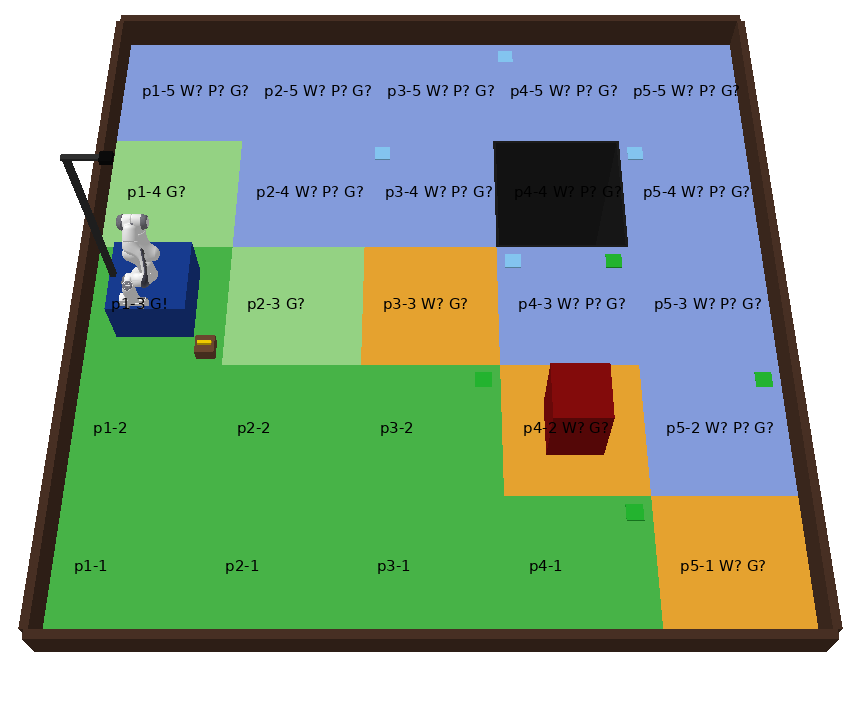
\includegraphics[width=\linewidth]{short/wumpus_explore_frame007.png}
  \caption{The rule explorer in the Wumpus world, at the gold after 16 actions.}
\end{subfigure}
\caption{The other settings of the tracks. Paths 7 and 8 work on (c), paths 2 and 7 on (d), paths 4 and 10 on (e).}
\label{fig:shots2}
\end{figure}

\begin{figure}[H]
\centering
\begin{subfigure}[t]{0.36\linewidth}\centering
\begin{tikzpicture}
\begin{axis}[sb, xbar stacked, bar width=9pt, width=\linewidth, height=3.3cm,
  xmin=0, xmax=80, xtick={0,20,40,60,80}, xlabel={pairs of one scene and repetition},
  ymin=0.4, ymax=2.6, ytick={1,2}, yticklabels={run 2,run 1},
  legend style={at={(0.5,1.04)}, anchor=south, legend columns=2},
  nodes near coords, nodes near coords style={font=\scriptsize},
]
\addplot[fill=black!60, draw=none, every node near coord/.append style={text=white}] coordinates {(37,1) (30,2)};
\addplot[fill=cours, draw=none, every node near coord/.append style={text=white}] coordinates {(18,1) (25,2)};
\addplot[fill=ctamp, draw=none, every node near coord/.append style={text=white}] coordinates {(9,1) (6,2)};
\addplot[fill=black!18, draw=none] coordinates {(12,1) (17,2)};
\legend{both, only ours, only TAMPURA, neither}
\end{axis}
\end{tikzpicture}
\caption{The pairs of \BF{63}. Run 2 decides: 18 to 9, exact McNemar $p = 0.12$. Run 1 ($p = 0.00088$) holds a slow hour of the cluster.}
\end{subfigure}\hfill
\begin{subfigure}[t]{0.30\linewidth}\centering
\begin{tikzpicture}
\begin{axis}[sb, ybar, bar width=11pt, width=\linewidth, height=3.9cm,
  ymin=0, ymax=128, ytick={0,50,100}, ylabel={successes (\%)},
  symbolic x coords={a,b,c,d}, xtick={a,b,c,d},
  xticklabels={{ours},{T, fixed},{T, hand B},{T, hand C}},
  x tick label style={font=\scriptsize, rotate=25, anchor=north east},
  enlarge x limits=0.2,
  nodes near coords, point meta=explicit symbolic,
  nodes near coords style={font=\scriptsize},
  ymajorgrids,
]
\addplot[fill=cours, draw=none, bar shift=0pt] coordinates {(a,100) [10/10]};
\addplot[fill=ctamp, draw=none, bar shift=0pt] coordinates {(b,60) [6/10]};
\addplot[fill=ctamp!45, draw=none, bar shift=0pt] coordinates {(c,100) [5/5] (d,50) [1/2]};
\end{axis}
\end{tikzpicture}
\caption{The mirror (path 5): TAMPURA's planner (T) on our scenes. The two hand-camera batches (pale) were cut short.}
\end{subfigure}\hfill
\begin{subfigure}[t]{0.30\linewidth}\centering
\begin{tikzpicture}
\begin{axis}[sb, ybar stacked, bar width=16pt, width=\linewidth, height=3.9cm,
  ymin=0, ymax=20, ytick={0,5,10,15,20}, ylabel={episodes of 20},
  symbolic x coords={a,b}, xtick=data,
  xticklabels={{four-fix set},{with limited accel.}},
  enlarge x limits=0.6,
  legend style={at={(0.5,1.04)}, anchor=south, legend columns=1},
  nodes near coords, point meta=explicit symbolic, nodes near coords style={font=\scriptsize},
  ymajorgrids,
]
\addplot[fill=vrerun, draw=none, every node near coord/.append style={text=white}] coordinates {(a,6) [6] (b,0) []};
\addplot[fill=black!70, draw=none, every node near coord/.append style={text=white}] coordinates {(a,3) [3] (b,4) [4]};
\addplot[fill=black!15, draw=none] coordinates {(a,11) [11] (b,16) [16]};
\legend{box lost to the swing, box lost to a collision, box kept}
\end{axis}
\end{tikzpicture}
\caption{TB-23, the dropped tall box: 40 headless probe episodes in two settings (path 3). A probe, not an evaluation.}
\end{subfigure}
\caption{The comparison's pairs, the mirror experiment, and the drop that the success counts do not see.}
\label{fig:pairs}
\end{figure}

\section{What was tested, and what stands}
\label{sec:tested}

For this version an audit read every evaluation, probe and check on record, 48 in all, and judged each against nine
criteria: one success test for all arms, drops and collisions recorded, Hani's visual check, approved deviations,
the same machine for all arms, the code version, the statistics, known bugs, and the match with published
settings. A second reader then checked the verdicts against the sources: it confirmed 43 points, corrected 19 and
found one unsupported, and this version follows its corrections. Fifteen records stand as reported (\vOK),
twenty-one stand for a narrower claim than version 2 makes (\vNA), two have to be run again (\vRE: one ran before
its deviations were approved, one was cut after 2 of 10 seeds), and ten were built or prepared and never ran.
\Cref{fig:timeline} shows when and where the runs took place; \Cref{tab:cluster} and \Cref{tab:laptop} list the
ones that carry a number of the report.

\begin{figure}[H]
\centering
{\scriptsize\setlength{\tabcolsep}{3pt}\renewcommand{\arraystretch}{1.1}%
\begin{tabularx}{\linewidth}{@{}>{\bfseries}p{0.95cm}*{8}{Y}@{}}
\toprule
 & \textbf{before 27 Oct} & \textbf{27 Oct} & \textbf{28 to 30 Oct} & \textbf{31 Oct to 2 Nov} &
   \textbf{3 and 4 Nov} & \textbf{6 Nov} & \textbf{7 Nov} & \textbf{8 Nov} \\
\midrule
cluster &
 &
\sq{vok}TAMPURA as shipped: 13 of 20\par \sq{vnarrow}our pipeline twice: 31 and 30 of 40 &
\sq{vnot}first two campaigns against TAMPURA: our arm void &
\sq{vnarrow}time cuts: 34.6 to 23.2\,s\par \sq{vnarrow}die-slip campaign: 120 of 120 against 40 of 60 &
\sq{vnarrow}run 1: a slow hour\par \sq{vnarrow}run 2: 57 of 80 against 46 of 76, $p = 0.12$ &
\multicolumn{3}{l}{\normalfont\emph{Nothing ran on the cluster during the tracks.}} \\
\midrule
laptop &
\sq{vnarrow}A/B of two perception fixes (18 Sept, the thesis's harness): 27 of 40 for both &
 &
\sq{vnarrow}squeeze probe: 0.5\,mm holds the die in 93 of 96 trials &
 &
\sq{vnarrow}shadow fix on scene 118: solved &
\sq{vok}check of the tag\par \sq{vnarrow}the mirror: 10 of 10 against 6 of 10 (to be repeated)\par
\sq{vnarrow}LW1 drives our robot: 18 of 18\par \sq{vnarrow}planning layer alone: 18 of 20 and 17 of 25\par
\sq{vnarrow}shadow fix, local check &
\sq{vok}walkers: the luck floor\par \sq{vnarrow}hand camera for the looks: 5 of 5\par
\sq{vrerun}hand camera for every image: cut at 2 of 10\par \sq{vrerun}path 7, first arm &
\sq{vnarrow}probes of the dropped box (TB-23)\par \sq{vok}merge checks of the Wumpus branch \\
\midrule
events &
\textcolor{darkgray}{10 June: thesis handed in. 20 Aug: the first bridge thrown away. 25 Oct: the restart.} &
 &
\textcolor{darkgray}{30 Oct: the squeeze of 0.5\,mm becomes the default.} &
\textcolor{darkgray}{2 Nov: the four slip switches on by default.} &
 &
\textcolor{darkgray}{The stable tag; the tracks start.} &
\textcolor{darkgray}{WSL wedges at 11:02; rule 15 at 13:22; no WSL work from 13:25.} &
\textcolor{darkgray}{Rule 18 (drops and collisions); Checkpoint 1: everything pauses.} \\
\bottomrule
\end{tabularx}}
\caption{What ran when and where. \sq{vok}stands as reported;\quad \sq{vnarrow}stands for a narrower claim;\quad
\sq{vrerun}has to be run again;\quad \sq{vnot}void. Every comparison with TAMPURA on its own task ran on the
cluster before the tracks; every run of the tracks ran on the laptop.}
\label{fig:timeline}
\end{figure}

\paragraph{Four findings cut across all of them.}
\emph{No old record can be re-scored for drops.} Telemetry was switched off in every evaluation, so the records hold
no ground truth about drops or collisions (TB-22). The old numbers will always be success by each arm's own test;
clean success needs new runs.
\emph{Every number of ours against TAMPURA rests on two end tests}, our goal check and TAMPURA's reward on its
belief. The shared test is built (\BF{70}) and has never run.
\emph{Whether rule 15 reaches back is open.} Hani's words of 7 November are ``the current ones can stay if i
confirm it is working out''. The die-slip campaign and the generated scenes had ended days before. Version 2 reads
them as run before the rule, the audit's first reader as current ones that need his confirmation. Both readings
are possible; it is a question for Hani, not a failed criterion.
\emph{The machines.} On the cluster the arms ran one after the other on one node; the exceptions are named in
\Cref{tab:cluster}. TAMPURA as shipped had an exclusive node; in run 2 the nodes were shared, each job with its own
cores, and three jobs waited for memory. On the laptop the
tracks shared one machine from 6 to 8 November, with waits of 23 to 44 minutes for the lock and a commit charge of
up to 95.1\,\%. No episode met a time cap there, so the load touches the times of these runs and not their counts.
The measured code is the right one: every commit behind the die-slip campaign and run 2 is an ancestor of the tag,
and run 2 differs from the tag in no pipeline file.

\begin{table}[H]
\centering\footnotesize
\begin{tabularx}{\linewidth}{@{}P{0.20\linewidth}P{0.205\linewidth}P{0.075\linewidth}Y@{}}
\toprule
evaluation & result as reported & verdict & what stands, and why not more \\
\midrule
TAMPURA as shipped, seeds 0 to 19 (27 Oct) & 13 of 20 & \vOK &
One system alone on an exclusive node. \\
The unchanged pipeline twice, our holding scene (27 Oct) & 31 and 30 of 40 & \vNA &
A noise floor for code older than the slip switches; $n = 40$. \\
Four time cuts, 8 arms on 24 seeds (31 Oct) & search settings: median wall 34.6 to 23.2\,s & \vNA &
A node shared with other users and code from before the slip switches. Only the ratio between arms holds (0.89 of
the base per seed); no absolute time can be quoted. \\
The die-slip campaign, three shipped scenes (31 Oct to 2 Nov) & chosen set 120 of 120; base 209 of 300; TAMPURA
40 of 60 & \vNA &
Stands for the three shipped layouts, each arm by its own end test, planner against planner, at a cap of 600\,s
per episode. ``No die lost'' is what the pipeline noticed, not a ground truth. \\
40 generated scenes, run 1 (3 Nov) & 57 of 80 against 36 of 78, $p = 0.00088$ & \vNA &
One slow hour of the cluster caused TAMPURA's timeouts; outside it $p = 0.21$. Not evidence of a significant lead. \\
40 generated scenes, run 2 (4 Nov) & 57 of 80 against 46 of 76; pairs 18 to 9; $p = 0.12$ & \vNA &
The strongest result: a design declared in advance, on the tag's code. Its limits: two end tests, no record of
drops, 76 pairs that carry about 38 draws, the clipped-shadow bug in our arm, and $p = 0.248$ once TAMPURA's
20-step budget is counted for ours. \\
Our runs of TAMPURA against its paper & return 0.530 against 0.63 $\pm$ 0.07 & \vNA &
Consistent with the paper, on other scenes and other hardware; four crashed runs are left out. The comparison of
times is not valid. \\
\bottomrule
\end{tabularx}
\caption{The evaluations on the chair's cluster. All ran before the tracks; nothing has run on the cluster since 4
November. The first two campaigns against TAMPURA (30 October) are void for our arm, which crashed on every episode.}
\label{tab:cluster}
\end{table}

\begin{table}[H]
\centering\footnotesize
\begin{tabularx}{\linewidth}{@{}P{0.20\linewidth}P{0.205\linewidth}P{0.075\linewidth}Y@{}}
\toprule
run & result as reported & verdict & what stands, and why not more \\
\midrule
The mirror: TAMPURA's planner on our scenes, fixed camera, ten seeds (path 5) & ours 10 of 10, TAMPURA 6 of 10 &
\vNA &
The setup was approved, so the run is valid, but TAMPURA's 6 of 10 is confounded: three of its four failures are
look loops, which the logs, as far as they were read, tie to our fixed camera. Hani's words of 7 November made its
own hand camera the setup, so the run is repeated. Its execution is kinematic. Ours' 10 of 10 very likely holds
drops: the same setting lost the box in 3 of 3 and 2 of 2 probe carries on seeds 3 and 4. \\
The same with TAMPURA's hand camera for its looks, five seeds & 5 of 5 & \vNA &
None of the three look-loop seeds is among the five, so the batch does not answer its question. \\
The same with the hand camera for every image & 1 of 2, then cut & \vRE &
Incomplete: two of ten seeds, cut by the stop order for WSL. \\
Our planning layer on \cuncert, 20 seeds (path 2) & their reward 18 of 20; world test 17 of 20 & \vNA &
The decision layer only, on TAMPURA's execution functions and object models. No TAMPURA arm ran in the same
conditions; the times are indicative. On seed 14 their reward is reached with no fruit in the bowl; the world
test catches it. \\
Our planning layer on \slamcol, 25 episodes (path 2) & their reward 17 of 25; world test 21 of 25 & \vNA &
A scripted rule reaches the same 17 of 25 and a second one 19, so the result does not show that planning adds
anything under their reward. Its deviations have no written approval. \\
\cuncert\ with boxels, first arm (path 7) & the same numbers as path 2 & \vRE &
It ran before Hani had approved its deviations; the rows are held back and carry no drop fields. \\
LW1 alone against its paper's Table 2 (path 4) & 100 of 100 at 5x5; 9.95 calls and 13.65 actions against 12.2 and
15.2 & \vNA &
Solved matches; calls and length miss the paper, likely because the code is the 2018 version. 10x10 rests on 3
states and 15x15 on 1. \\
LW1 drives our robot, 18 episodes (path 4) & 18 of 18; 0 of 369 percepts wrong & \vNA &
10, 5 and 3 states at 5x5, 7x7 and 10x10; the base is placed kinematically; collisions were not detected. \\
Walkers on LW1's states, grid code (path 10) & the luck floor of the test & \vOK &
At 5x5 the floor is 34 to 39.5\,\%: the random walk wins more than the frontier walker. \\
The probes of the dropped box, 52 episodes (TB-23) & swing losses 6 of 20 against 0 of 20 & \vNA &
A probe with 2 to 6 repetitions per seed and setting; 20 of the 52 episodes ran without telemetry, their causes
come from the logs. Collisions remain with the cure (4 of 20). \\
The shadow fix, local check (\BF{64}) & 18 seeds, no regression & \vNA &
14 seeds were scored (4 stopped at a gate), and no arm of the tag ran beside them. The measurement is the
cluster's arm with the fix. \\
\bottomrule
\end{tabularx}
\caption{The runs of the tracks on the laptop, 6 to 8 November, in WSL under the pipeline lock. Also valid as
recorded: the replay of LW1's percepts on the robot (no mismatch), the random baselines, the recount of the thesis's
timeouts, the finding of \BF{65}, the check of the tag and the test suites.}
\label{tab:laptop}
\end{table}


\paragraph{Corrections to version 2.} Its sentence that nothing has run on the cluster holds only for the tracks
since 6 November. The luck floor at 5x5 is 34 to 39.5\,\%, not about a third. The local check of the shadow fix
scored 14 seeds, not 18. The die-slip campaign ran with a cap of 600\,s per episode; the 900\,s that version 2
gives for both arms hold for the generated scenes. And the acceleration-limited carry cost a factor of 1.22 in
execution time on \fdice\ (\BF{59}) but nothing measurable per carry in the probes of TB-23: these are two
measures, not one claim.

\begin{figure}[H]
\centering
\begin{subfigure}[t]{0.215\linewidth}\centering
  \includegraphics[width=\linewidth]{\arch/tracks/reverse/batch_hand_c/first_views/probe_s9_first_view_fixed.png}
  \caption{Seed 9 at the start, through our fixed camera: the target is hidden behind the two boxes.}
\end{subfigure}\hfill
\begin{subfigure}[t]{0.215\linewidth}\centering
  \includegraphics[width=\linewidth]{\arch/tracks/reverse/batch1/failed_T/s9_final_view.png}
  \caption{Seed 9 at the end of TAMPURA's run with that camera: 20 looks, no pick, nothing has moved.}
\end{subfigure}\hfill
\begin{subfigure}[t]{0.215\linewidth}\centering
  \includegraphics[width=\linewidth]{\arch/tracks/reverse/batch_hand_c/first_views/probe_s9_first_view_hand.png}
  \caption{The same start through TAMPURA's own hand camera: the target (orange) is in view between the boxes.}
\end{subfigure}\hfill
\begin{subfigure}[t]{0.215\linewidth}\centering
  \includegraphics[width=\linewidth]{\arch/tracks/reverse/batch1/failed_T/s7_SUCCESS_final_view.png}
  \caption{Seed 7, one of TAMPURA's six successes: an occluder moved aside, the target (blue) in the hand.}
\end{subfigure}
\caption{Why the mirror has to be repeated. The camera decides what TAMPURA's planner can find out by looking, so
its 6 of 10 measures our fixed camera as much as its planning. With the hand camera for every image seed 9 needs
no look at all, so the two hand-camera variants answer different questions.}
\label{fig:mirror}
\end{figure}

\section{Re-runs and pending tests: laptop only, or cluster}
\label{sec:placement}

Three reasons put a test on the laptop: Hani has to watch it; its code and builds exist only in the laptop's WSL;
or its numbers will stand beside numbers that were measured on the laptop. Every comparison whose number or time
goes into the paper belongs on the cluster, and only after Hani's yes to that question alone
(\Cref{tab:placement} and \Cref{tab:cluster-next}). The workable standard there is the design of run 2: one node type, TAMPURA and then ours
per scene on the same node, the episode folders on the node's own disk. Exclusive nodes cannot be counted on: on
4 November all 16 nodes were shared and 221 jobs waited. On the laptop no batch may start above a commit charge of
85\,\% (rule 14); at the pause it stood at 92 and 86\,\%, so every laptop item below waits for memory first.

\begin{table}[H]
\centering\footnotesize
\begin{tabularx}{\linewidth}{@{}P{0.40\linewidth}P{0.17\linewidth}Y@{}}
\toprule
test & size & why there, and what it needs first \\
\midrule
Hani's visual checks under rule 15, in one round: the mirror (TAMPURA's hand camera on seeds 3 and 4, 4 to 11
minutes a seed), the cluster waves, \cuncert\ (seeds 0 and 13), the Wumpus arms, the look action &
at least four GUI runs per comparison, six each for paths 9 and 10, started by Hani &
They need Hani's display. A window shows behaviour, not the cluster's times, and a laptop run of a shipped
\fdice\ seed loads another scene than the cluster's run of that seed. \\
The drop cure: Hani's look at seeds 3 and 4 with and without the acceleration-limited carry, the A/B of three
arms, then the die on \fdice\ re-checked with the switch &
two commands; then about 170 episodes, 50 minutes &
It counts losses inside one batch and decides only the default. \\
The mirror again: the eight remaining seeds with TAMPURA's hand camera for every image &
40 to 90 minutes &
The glue runs only in WSL, and the result is compared only with laptop numbers. First: the check under rule 15.
Ours again with drop counts needs Go's or Hani's word: the order is to keep its ten rows. \\
The hand camera for the looks only, on the five seeds left (6, 7, 9, 10, 11), if Hani wants them &
about 25 minutes &
The only design that tests the look loops on the look-loop seeds with the first view unchanged. \\
The first real run of the shared success test: one TAMPURA episode and three tests against the real package; the
last check of the job scripts and a smoke of every snapshot &
minutes (about 3 on the cluster; no laptop time is on record) &
The gate before any wave on the cluster. The first campaigns crashed on a line that their smoke never reached. \\
The cost of the drop counts (TB-22) on a few seeds, with and without &
minutes &
Repeated on the cluster's node type if it exceeds about 1\,\%. \\
The clean \cuncert\ batch (path 7) &
about 45 minutes &
Compared with path 2's rows, which are laptop rows. \\
LW1 alone on all 100 states at 10x10, the replay at 15x15, and the required sets of our setup in the Wumpus world &
35 minutes; about 2 hours &
The patched LW1 build exists only in WSL, and path 4's runs are laptop runs. \\
Development runs: the look action's smokes and three arms on the tabletop, the random baselines of path 2, the
first episodes of path 8, the install for path 15 &
75 minutes; under 30; open &
No number for the paper comes from them. \\
\bottomrule
\end{tabularx}
\caption{The tests that have to run on the laptop, and only there. Builds, unit tests, the test suites of the
merges and recounts from existing records can run anywhere.}
\label{tab:placement}
\end{table}

\begin{table}[H]
\centering\footnotesize
\begin{tabularx}{\linewidth}{@{}P{0.40\linewidth}P{0.17\linewidth}Y@{}}
\toprule
test & size & why there, and what it needs first \\
\midrule
Wave 1 of path 6: our code now against the thesis code on our tabletop &
270 cells per arm, 1\,800\,s per cell &
A wall-clock budget, so both arms on one node type. \\
Wave 2 of path 6: ours, ours with the shadow fix, and TAMPURA on 200 fresh \fdice\ scenes, with the shared success
test, TAMPURA's 20-action cap on ours and the drop counts &
900\,s per episode; the two waves about 53 node-hours &
The paper's replacement for the 40 generated scenes. First: TB-22, the local run of the shared test, rule 15. \\
TAMPURA on our tabletop with ours in the same jobs (phase 2 of path 6) &
90 cells &
The laptop times of the mirror cannot stand beside cluster times. First: path 5's merge. \\
The shipped scenes again with clean success, if the paper keeps that claim &
seeds 0 to 19 three times; ours about 1.5 hours, TAMPURA about 3 &
The die-slip campaign cannot be re-scored. The cap (600 or 900\,s) has to be chosen. \\
TAMPURA on \cuncert, seeds 0 to 19, with 20 seeds of an arm of ours in the same job (Q42; which arm is not
decided); the \slamcol\ pilot (Q44) &
about 3.4 hours; up to 4 hours &
Only then does the planning layer have a TAMPURA arm in the same conditions. \\
\bottomrule
\end{tabularx}
\caption{The tests that belong on the cluster, each after Hani's yes to that question alone.}
\label{tab:cluster-next}
\end{table}

\paragraph{Numbers that must not stand side by side.} The laptop medians of the mirror (16.4\,s for ours,
250.2\,s for TAMPURA) and any cluster time; the local check of the shadow fix and run 2; the absolute times of the
time cuts and anything else (their ratios can be quoted); LW1's times and its paper's (calls and lengths compare);
TAMPURA's published time per step, measured on a Xeon Gold 6248, and the times of our cluster's Xeon Platinum 8160;
a laptop run and a cluster run of the same shipped \fdice\ seed, because the two machines list the scene files in
another order (a per-seed comparison with the thesis holds for seven seeds only).

\paragraph{The order.} \Cref{fig:route} gives the order in which the re-runs and the pending tests unblock each
other. Three notes on it. Step 3 includes the decision whether path 14's fix for the carry into unseen space
enters the paper's code. Step 7 covers the \slamcol\ lists, path 9's items and path 8's rounds, and a word on the
pad tolerance of 2\,mm in the shared test, which is the building session's reading and not Hani's. For step 9,
Hani's yes of 7 November (about 53 node-hours) is on record; the tracks' state asks the question again, alone,
after rule 15, and path 6's files only if the node-hours change.

\begin{figure}[H]
\centering
\begin{tikzpicture}[>=stealth,
  st/.style={draw=black!45, rounded corners=1.5pt, font=\scriptsize, text width=2.42cm, minimum height=1.58cm,
             align=left, inner sep=2.5pt, anchor=north west},
  hani/.style={st, fill=ctamp!20}, lap/.style={st, fill=cours!13}, clu/.style={st, fill=black!14},
  ar/.style={->, black!60, line width=0.6pt}]
\node[hani] (a1) at (0,0)      {\textbf{1}\ \ Hani watches ours on seeds 3 and 4, with and without the acceleration-limited carry, and gives the OK};
\node[lap]  (a2) at (2.975,0)  {\textbf{2}\ \ The A/B of the drop cure (about 170 episodes, 50 minutes); the die re-checked on \fdice};
\node[hani] (a3) at (5.95,0)   {\textbf{3}\ \ Hani decides the default of the carry};
\node[lap]  (a4) at (8.925,0)  {\textbf{4}\ \ The drop and collision counts (TB-22): built, their cost measured; about a day};
\node[lap]  (a5) at (11.9,0)   {\textbf{5}\ \ The merges; the three hunks cleaned out of the main checkout};
\node[lap]  (a6) at (14.875,0) {\textbf{6}\ \ The paper's code frozen and tagged, with its own check};
\node[hani] (b1) at (0,-2.0)      {\textbf{7}\ \ Hani's open approvals (rule 12) and visual checks (rule 15), in one round};
\node[lap]  (b2) at (2.975,-2.0)  {\textbf{8}\ \ The first real run of the shared success test; a smoke of every snapshot};
\node[hani] (b3) at (5.95,-2.0)   {\textbf{9}\ \ The cluster question};
\node[clu]  (b4) at (8.925,-2.0)  {\textbf{10}\ \ Wave 1 and wave 2: about 53 node-hours, 9 to 13 hours from the go to the numbers};
\node[lap]  (b5) at (11.9,-2.0)   {\textbf{11}\ \ The laptop comparisons, one batch at a time: the mirror, \cuncert, the Wumpus runs};
\node[hani] (b6) at (14.875,-2.0) {\textbf{12}\ \ The recounts and the tables of clean success; Hani picks the headline criterion};
\foreach \a/\b in {a1/a2, a2/a3, a3/a4, a4/a5, a5/a6, b1/b2, b2/b3, b3/b4, b4/b5, b5/b6} {\draw[ar] (\a.east) -- (\b.west);}
\draw[ar] (a6.south) -- ++(0,-0.2) -| (b1.north);
\end{tikzpicture}
\caption{The order of the next steps. Orange: Hani acts. Blue: an agent on the laptop. Grey: the cluster. The
last start of the evaluation campaign is 24 November, the paper's deadline 4 December (\BF{1}).}
\label{fig:route}
\end{figure}

\section{What stopped right before it was done}
\label{sec:stopped}

The checkpoint halted every batch on 8 November. \Cref{fig:tracks} shows how far each track got, and
\Cref{tab:stopped} lists what was within one step of a result.

\begin{figure}[H]
\centering
\begin{subfigure}[t]{0.52\linewidth}\centering\footnotesize
\renewcommand{\arraystretch}{1.0}
\begin{tabular}[t]{@{}rl@{\hspace{5pt}}c@{\hspace{7pt}}c@{\hspace{7pt}}c@{\hspace{7pt}}c@{\hspace{7pt}}c@{}}
\toprule
 & path & built & tests & episodes & result & merged \\
\midrule
1 & drawing in the GUI & \dY & \dY & \dY & \dY & \dH \\
2 & two other TAMPURA tasks & \dY & \dN & \dY & \dH & \dN \\
3 & bug board and fixes & \dY & \dY & \dY & \dH & \dH \\
4 & LW1 in the Wumpus world & \dY & \dY & \dY & \dH & \dN \\
5 & TAMPURA on our scenes & \dY & \dY & \dY & \dH & \dN \\
6 & cluster evaluation & \dY & \dY & \dH & \dN & \dN \\
7 & planning layer with boxels & \dY & \dY & \dH & \dN & \dN \\
8 & \cuncert\ in our setup & \dH & \dY & \dN & \dN & \dN \\
9 & one look action & \dY & \dY & \dN & \dN & \dN \\
10 & our setup in the Wumpus world & \dY & \dH & \dH & \dH & \dN \\
14 & collision and drop detection & \dN & \dN & \dN & \dN & \dN \\
15 & SS-Replan feasibility & \dN & \dN & \dN & \dN & \dN \\
\bottomrule
\end{tabular}
\caption{The tracks by stage. \dY\ yes;\ \dH\ in part;\ \dN\ no. Result: full if it stands as reported, half if
it stands for a narrower claim or a part, empty if there is none or a re-run is needed. Path 6's episodes are a
local smoke only. Paths 11 to 13 are reports and are done.}
\end{subfigure}\hfill
\begin{subfigure}[t]{0.45\linewidth}\centering
\begin{tikzpicture}[baseline=(current bounding box.north)]
\begin{axis}[sb, xbar, bar width=6pt, width=0.74\linewidth, height=4.5cm,
  xmin=0, xmax=13, xtick={0,2,4,6},
  xlabel={bugs of 23},
  symbolic y coords={theirs,launcher,merged,latent,fixed,open,hani},
  ytick={theirs,launcher,merged,latent,fixed,open,hani},
  yticklabels={{in TAMPURA's code},{fixed in the launcher},{merged},{analysed or latent, no fix},{fixed, waits for the merge},{open},{waits for Hani's choice}},
  enlarge y limits=0.1,
  nodes near coords, point meta=explicit symbolic,
  nodes near coords style={font=\scriptsize, anchor=west},
  xmajorgrids,
]
\addplot[fill=black!50, draw=none] coordinates {(1,theirs) [TB-19] (1,launcher) [TB-10] (1,merged) [TB-16] (4,latent) [TB-11, 12, 15, 18] (4,fixed) [TB-1, 8, 17, 20] (6,open) [TB-9, 13, 14, 21 to 23] (6,hani) [TB-2 to TB-7]};
\end{axis}
\end{tikzpicture}
\caption{The bug board of path 3 at the checkpoint. TB-22 is the missing drop record, TB-23 the dropped box.}
\end{subfigure}
\caption{How far the tracks got, and where the 23 bugs stand.}
\label{fig:tracks}
\end{figure}

\paragraph{Stopped, but far from done.}
\emph{The cluster evaluation} (path 6) has its plan, its job scripts and Hani's yes of 7 November, but nothing is
pushed: the local run of the shared test, the check under rule 15, the snapshots, a smoke and two waves of about
53 node-hours remain.
\emph{\cuncert\ in our setup} (path 8) lacks its driver and every batch; Hani's Rounds 2 and 3 are open, and the
first numbers are about 12 working days out.
\emph{The drop counts} (TB-22) have a chosen design and no code.

\begin{figure}[H]
\centering
\begin{subfigure}[t]{0.25\linewidth}\centering
  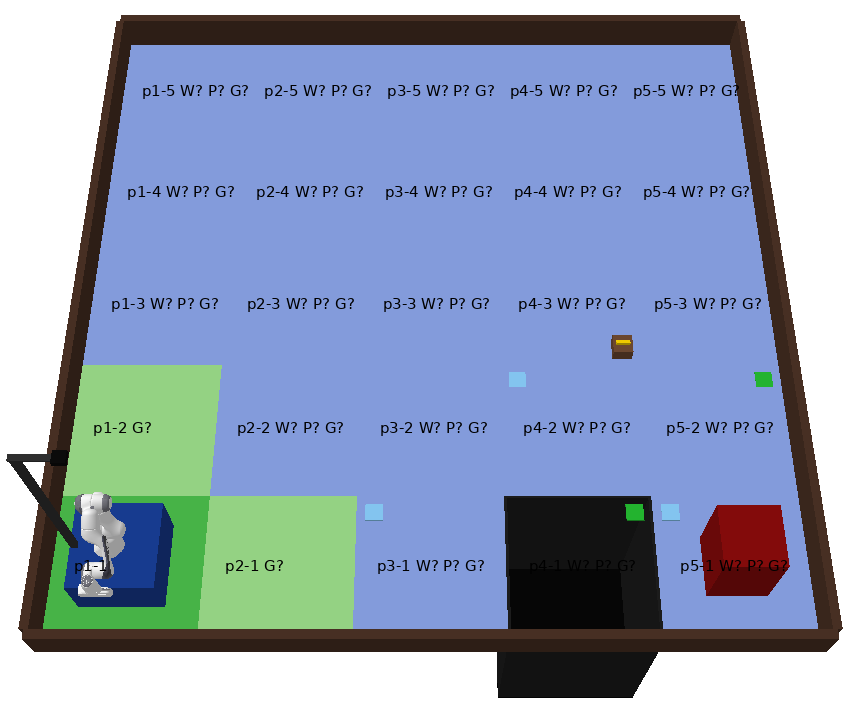
\includegraphics[width=\linewidth]{short/wumpus_lw1_frame000.png}
  \caption{LW1 drives our robot, hidden state 0 at 5x5, after 1 action: 3 tiles safe, 22 may hold a pit.}
\end{subfigure}\hfill
\begin{subfigure}[t]{0.25\linewidth}\centering
  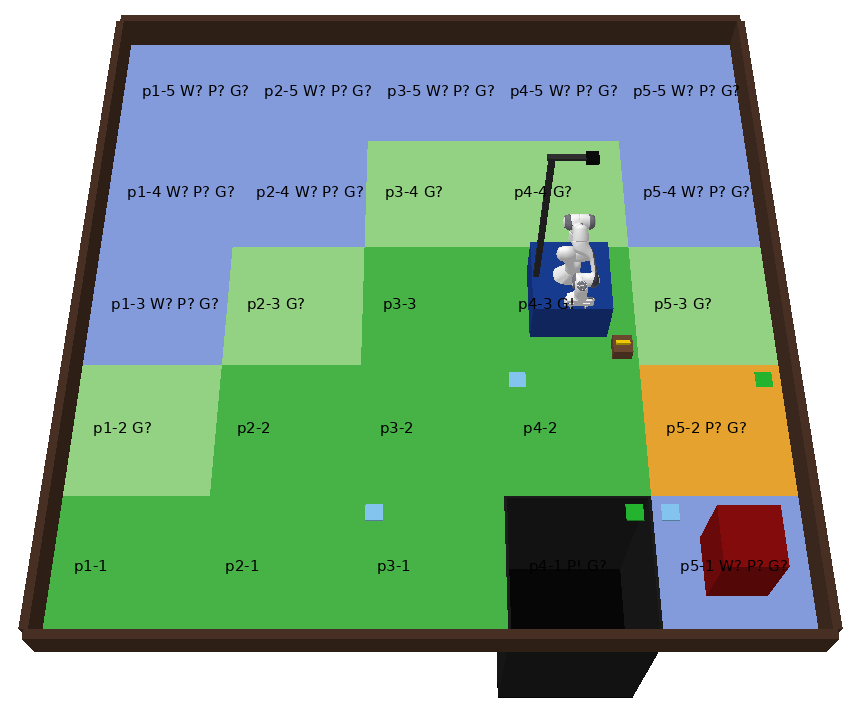
\includegraphics[width=\linewidth]{short/wumpus_lw1_frame009.png}
  \caption{The same run after 19 actions: 8 tiles visited, 13 safe, the gold known.}
\end{subfigure}\hfill
\begin{subfigure}[t]{0.25\linewidth}\centering
  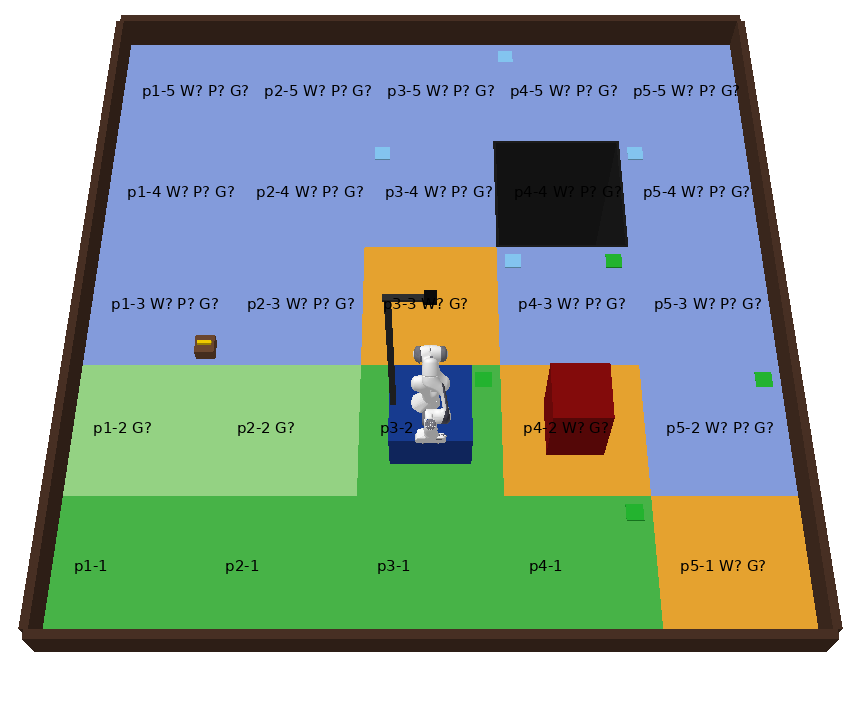
\includegraphics[width=\linewidth]{short/wumpus_explore_frame004.png}
  \caption{The rule explorer on another state after 10 actions: 5 tiles visited, 7 safe.}
\end{subfigure}\hfill
\begin{minipage}[b]{0.19\linewidth}\scriptsize\color{darkgray}\raggedright
  \textbf{Tile colours}\par\vspace{2pt}
  \textcolor[RGB]{134,157,220}{\rule{1.6ex}{1.6ex}}\ nothing known\par
  \textcolor[RGB]{232,163,53}{\rule{1.6ex}{1.6ex}}\ one hazard ruled out\par
  \textcolor[RGB]{150,214,130}{\rule{1.6ex}{1.6ex}}\ both hazards ruled out\par
  \textcolor[RGB]{70,178,70}{\rule{1.6ex}{1.6ex}}\ visited\par
  \textcolor[RGB]{200,50,50}{\rule{1.6ex}{1.6ex}}\ a hazard known\par\vspace{3pt}
  The black shaft is the pit, the dark red box the Wumpus, the bar on a pedestal the gold.\par\vspace{14pt}
\end{minipage}
\caption{The painter of the Wumpus world (path 4), whose look by Hani the merge of the Wumpus branch waits for. It
paints on each tile what the planner knows at that step. Off-screen renders of the merge checks of 8 November; the
framing and the label size in the GUI itself are not checked.}
\label{fig:painter}
\end{figure}

\begin{table}[H]
\centering\footnotesize
\begin{tabularx}{\linewidth}{@{}P{0.20\linewidth}P{0.27\linewidth}Y P{0.19\linewidth}@{}}
\toprule
item & where it stands & the step that is left & waits for \\
\midrule
The A/B of the acceleration-limited carry (TB-23, path 3) &
Prepared: three arms, about 170 episodes, 50 minutes; the script is written &
Run it; then Hani decides the default &
Hani's look at seeds 3 and 4 with and without the switch, and the written OK \\
TAMPURA with its own hand camera on our scenes (path 5, option C) &
2 of 10 seeds done when the stop order for WSL cut the batch on 7 November at 13:48 &
The other 8 seeds, 40 to 90 minutes of the laptop &
Hani's watch of the hand camera on seeds 3 and 4, then his written approval under rule 15 \\
Four fixes: TB-1, TB-8 with TB-20, TB-17 (path 3) &
Built, tested and reviewed; the merge requests are sent &
Go's check and merge; for TB-17 one lock rule has to win &
Go \\
The camera views in the GUI (path 1) &
Merge request sent; the code is byte-identical to the checked commit &
One re-run of the tests, then the merge. The tracks' state also asks for a pair of runs on seed 106; the path's
own file says that pair was dropped &
Go \\
The Wumpus branch (path 4) &
Merge checks passed (269 tests, 96 bridge tests, replay 48 of 48); the request is ready and not sent &
Send, check, merge &
Hani's look at the painter (\Cref{fig:painter}); Go \\
One success test for both arms (\BF{70}, path 6) &
Built, reviewed, checked against fake packages; never run on TAMPURA's real world &
One local TAMPURA episode (minutes) and three tests against the real package &
A free slot under the memory guard \\
\cuncert\ with boxels (path 7) &
The first arm ran and its rows are held back; the clean batch is ready &
Seeds 0 to 2 against path 2's rows &
Rule 15 on seeds 0 and 13 \\
The single look action (path 9) &
Both looks built, 238 tests pass, no episode &
Two smokes, eight development seeds, then three arms on the tabletop, 75 minutes &
Hani's items 1, 2, 7 and Q-L1 to Q-L3 \\
Our setup in the Wumpus world (path 10) &
Three arms built and unit-tested; nothing run &
Merge the Wumpus tip in, the robot tests, the required sets, about 2 hours &
Path 4's merge; rule 15 \\
\bottomrule
\end{tabularx}
\caption{Work that stopped one step short. Smaller items of the same kind: LW1 alone on all 100 states at 10x10
(35 minutes, Hani's item b of path 4), the random baselines of path 2 (under 30 minutes), and the fix TB-9 (not built).}
\label{tab:stopped}
\end{table}

\section{What is still missing}
\label{sec:missing}

The paper's deadline is 4 December 2026, and the last start of the evaluation campaign is 24 November (\BF{1}).

\begin{figure}[H]
\centering
\tile{vok}{102}{solved with the fix}\hfill
\tile{vok}{103}{solved with the fix}\hfill
\tile{vok}{107}{solved with the fix}\hfill
\tile{vok}{111}{solved with the fix}\hfill
\tile{vok}{118}{solved with the fix}\hfill
\tile{vok}{127}{solved with the fix}\par\vspace{3pt}
\tile{vrerun}{100}{the shadow is a sliver of 2.3\,cm and is seen empty}\hfill
\tile{vrerun}{128}{the reach gate refuses the shadow's centre}\hfill
\tile{vrerun}{135}{the reach gate refuses the shadow's centre}\hfill
\tile{vrerun}{104}{the die lies tilted in view, 6 pixels, and no look can see it}\hfill
\tile{vrerun}{101}{the grasp fit rejects every wrist look of a far cup}\hfill
\tile{vrerun}{124}{a look and pick loop on a far cup, to the time cap}
\caption{The 12 generated scenes on which ours fails in both runs: the end of the failed episode of run 2
(repetition 0), the die ringed in red. Green frame: the scene succeeds in the local reruns with the fix for the
clipped shadow (\BF{64}). Red frame: it still fails, for the cause named (\BF{65}). In all 12 the die sits under
a cup, in none of our hiding regions. A local check on the laptop; the fix has no cluster run yet.}
\label{fig:gallery}
\end{figure}

\begin{itemize}
\item \textbf{Clean success.} No record of our pipeline counts drops or collisions (TB-22), and the detectors that
would feed the counts are path 14, which has not started. Until both exist, a success of ours may hide a drop.
\item \textbf{One success test for both arms.} It is built (\BF{70}) and has never run.
\item \textbf{A frozen code version for the paper.} The comparisons measured the tag; the shadow fix, the
acceleration-limited carry and path 14 would each change our arm, and the main checkout carries uncommitted hunks.
\item \textbf{Hani's written approval under rule 15.} None is on record for any comparison, and whether the rule
reaches back to the two finished comparisons is open.
\item \textbf{A significant or replicated comparison on fresh scenes.} Run 2 gave $p = 0.12$ on about 38 effective
pairs; the 200 scenes of the cluster's wave 2 are the planned answer.
\item \textbf{The cluster comparison} of our code now, the thesis code and TAMPURA, on the tabletop and on 200 fresh
\fdice\ scenes (path 6), with the fix for the clipped shadow as its own arm.
\item \textbf{The slip fixes on our own scenes.} They were measured on the die, on 40\,mm cubes and on a cup. On
our scenes the four-fix set lost tall boxes that the setting without the fixes kept (seed 3: 3 of 3 against 0 of
3). The acceptance of the 0.5\,mm squeeze on our scenes was not run either (\BF{44}).
\item \textbf{A decision on the die under the cup} (\BF{65}): a hiding region under objects, narrow fixes, or a
stated limitation in the paper (\Cref{fig:gallery}).
\item \textbf{TAMPURA itself on \cuncert\ and \slamcol} (cluster questions Q42 and Q44), and what the paper may say
from runs of the planning layer alone (Q45).
\item \textbf{Any result of our own setup} in the Wumpus world, with the look action, and on \cuncert\ in our setup.
\item \textbf{The cause of the WSL wedge} (\BF{69}), and a stop rule for the memory guard: its gate of 85\,\%
guards only a batch's start, and a batch that started at 84\,\% of the commit limit peaked at 95.1\,\%.
\end{itemize}


\begin{figure}[H]
\centering
\begin{subfigure}[t]{0.50\linewidth}\centering
\begin{tikzpicture}
\begin{axis}[sb, width=\linewidth, height=4.0cm,
  xmin=4, xmax=26, xtick={5,7,10,15,20,25}, xticklabels={5x5,7x7,10x10,15x15,20x20,25x25},
  ymin=0, ymax=108, ytick={0,25,50,75,100},
  xlabel={LW1's Wumpus states by grid size}, ylabel={wins of 100 states},
  legend style={at={(0.5,1.03)}, anchor=south, legend columns=3},
  ymajorgrids,
]
\addplot[black!70, thick, mark=square*, mark size=1.4pt] coordinates {(5,100) (7,100) (10,100) (15,100) (20,64) (25,43)};
\addplot[cours, only marks, mark=o, mark size=2.6pt, thick] coordinates {(5,100) (10,100) (15,100)};
\addplot[ctamp, thick, mark=*, mark size=1.3pt] coordinates {(5,39.5) (7,26.1) (10,21.9) (15,12.9) (20,6.6) (25,4.2)};
\addplot[vrerun, thick, mark=triangle*, mark size=1.6pt] coordinates {(5,34) (7,21) (10,24) (15,15) (20,9) (25,2)};
\addplot[black!45, thick, dashed, mark=x, mark size=2pt] coordinates {(5,33) (7,20) (10,10) (15,11) (20,8) (25,4)};
\legend{rule explorer, LW1 (published), random walk, frontier walker, straight line}
\end{axis}
\end{tikzpicture}
\caption{The luck floor of the Wumpus test (path 10): walkers that do not reason win 34 to 39.5\,\% of the 5x5 states. Our own setup has no result there.}
\end{subfigure}\hfill
\begin{subfigure}[t]{0.46\linewidth}\centering
\begin{tikzpicture}
\begin{axis}[sb, ybar, bar width=9pt, width=\linewidth, height=4.0cm,
  ymin=0, ymax=1.3, ytick={0,0.25,0.5,0.75,1}, ylabel={mean discounted return},
  symbolic x coords={cu,sl}, xtick=data,
  xticklabels={{\cuncert},{\slamcol}},
  enlarge x limits=0.5,
  legend style={at={(0.5,1.03)}, anchor=south, legend columns=1},
  nodes near coords, nodes near coords style={font=\scriptsize, rotate=90, anchor=west,
    /pgf/number format/fixed, /pgf/number format/precision=3},
  ymajorgrids,
]
\addplot[fill=ctamp, draw=none] coordinates {(cu,0.87) (sl,0.81)};
\addplot[fill=cours, draw=none] coordinates {(cu,0.788) (sl,0.567)};
\addplot[fill=cours!45, draw=none] coordinates {(cu,0.744) (sl,0.693)};
\legend{TAMPURA as published, our planning layer by their reward, our planning layer by the world-state test}
\end{axis}
\end{tikzpicture}
\caption{Two other TAMPURA tasks, the planning layer alone (path 2): their execution functions act, none of our perception or execution runs. TAMPURA itself was not run by us.}
\end{subfigure}
\caption{The Wumpus world and the two other tasks.}
\label{fig:other}
\end{figure}

\section{What can be achieved quickly}
\label{sec:quick}

\textbf{With less than an hour of Hani's time.}
\begin{enumerate}
\item Watch ours on seeds 3 and 4 with and without the acceleration-limited carry
(\texttt{run boxels -Seed 3,4 -Args '-{}-slip-fixes default,carry\_trapezoid'} and \texttt{run boxels -Seed 3,4}),
and give the OK. The A/B then runs in 50 minutes and the default can be decided.
\item Watch TAMPURA with its hand camera on seeds 3 and 4 of path 5 (4 to 11 minutes a seed), then write the
approval under rule 15. This comes after the decision on the drop cure, because what Hani's runs of ours showed
there was the dropped box. The eight seeds with TAMPURA's hand camera can then run.
\item Answer the decisions of \Cref{tab:decisions} in one round.
\item Look once at the Wumpus painter and at the camera viewer, each in a run that Hani starts.
\end{enumerate}

\begin{table}[H]
\centering\footnotesize
\begin{tabularx}{\linewidth}{@{}Y P{0.34\linewidth}@{}}
\toprule
decision that waits for Hani & what it unblocks \\
\midrule
The default of the acceleration-limited carry, after the look and the A/B & the paper's code and every later run of ours \\
The headline criterion, success or clean success, once the first counts are in (rule 18) & how every table of the paper is scored \\
Rule 15: the written approval for the mirror after the two watch runs, and whether the rule reaches back to the
die-slip campaign and the generated scenes & the hand-camera seeds; keeping the two comparisons \\
The die under the cup (\BF{65}): a hiding region under objects, the narrow fixes TB-2 to TB-6, or a stated
limitation & what the paper may claim for the occlusion model \\
The cluster question of path 6 (his yes of 7 November is on record; whether it is asked again is not settled
between the files); after it Q42 and Q44 & the two waves; a TAMPURA arm on the two other tasks \\
The open approvals under rule 12: the \slamcol\ lists with path 7's Q3; a word on the pad tolerance of 2\,mm in
the shared test; whether ours is run again in the mirror & any \slamcol\ run, the shared test, the mirror's drop counts \\
Path 9's items 1, 2, 7 and Q-L1 to Q-L3; path 8's Rounds 2 and 3 and its apple & the first episodes of the look action; path 8's batches \\
Path 4: sending the drafted question to LW1's authors (a), LW1 on all states at 10x10 (b), what to run at 15x15 (c) & the miss against the paper's Table 2 \\
Q45: what the paper may say from runs of the planning layer alone; path 12's four questions, path 13's deletions,
the priority of the camera viewer's window & a secondary table of the paper; 21.3\,GB of disk; the close of the
WSL report \\
\bottomrule
\end{tabularx}
\caption{The decisions that wait for Hani, most blocking first.}
\label{tab:decisions}
\end{table}
\textbf{With under a day of agent time each} (est.\ marks an estimate of the audit; the other efforts are stated
in the tracks' files).
\begin{itemize}
\item The merges: TB-8 with TB-20 and TB-1 (half a day with the tests and a locked episode, est.), the camera
views (a test hour, est.), TB-17 once the lock rule is chosen, and the Wumpus branch.
\item The first real run of the shared success test: one local TAMPURA episode and three package tests.
\item The drop and collision counts in our pipeline (TB-22, counts only): about a day with its timing runs (est.).
\item LW1 alone on all 100 states at 10x10 (35 minutes); the random baselines of path 2 (under 30 minutes); TB-9
(under two hours, est.); the clean \cuncert\ batch on seeds 0 to 2 (about 45 minutes).
\item The deletion of the dead pip folders, minutes after Hani's yes; step 1 of path 15, half a day to a day
(est.; no paper item, since any change to the pipeline from it waits until after the deadline).
\end{itemize}

\end{document}
